\documentclass[11pt,a4paper]{article}
\usepackage[utf8x]{inputenc}
\usepackage{graphicx}
\newcommand{\myincludegraphics}[2][]{% 
	\begingroup\setlength{\fboxsep}{0pt}% 
	\fbox{\includegraphics[#1]{#2}}% 
	\endgroup} 
\usepackage{esdiff}
\usepackage[english]{babel}
\usepackage{color}
\usepackage{booktabs}
\usepackage{tabularx}	
\usepackage{float}
\usepackage{enumitem}
\usepackage{epstopdf}
\usepackage{afterpage}
\usepackage{caption}
\usepackage{subcaption}
\captionsetup[table]{oneside , margin = {2cm, 0cm},
	justification=RaggedRight, singlelinecheck = false }
\usepackage{subcaption}
\usepackage{mathtools}
\usepackage{multicol}
\usepackage{algorithm2e}
\usepackage{microtype}
\usepackage{titling}
\usepackage{amsmath}
\usepackage{verbatim}
\usepackage{tasks}
\usepackage[hidelinks]{hyperref} % the option is there to remove the square around links which is what I don't like.
\usepackage{comment}
\usepackage{perpage} 
\MakePerPage{footnote} % Reset the footnote counter perpage. may require to run latex twice.
\usepackage{commath} % for absolute value
\usepackage[margin=2cm]{geometry} % This is here to fit more text into the page.

\setcounter{secnumdepth}{1}  % This removes the numbering from the subsections.
% If you want the numbering of the subsection level just remove this line
\usepackage{titling}
\newcommand{\subtitle}[1]{%
	\posttitle{%
		\par\end{center}
	\begin{center}\large#1\end{center}
	\vskip0.5em}%
}

\setlength{\parindent}{0pt} % No indentation for paragraphs. Because that is just old.
\setlength{\parskip}{\baselineskip} % Instead use vertical paragraph spacing.

\fontencoding{T1} % the better font encoding.
\title{\textsc{Optional Lab exercises}}
\subtitle{\textsc{Mechanical vibrations}}	
%\date{11/06/2020}
\author{Giorgio Checola}

\makeatletter
\def\@maketitle{
\graphicspath{ {./images/} }
\begin{center}
	
\includegraphics[width=75mm]{images/Unitn.png} \\
	\vspace{10mm}
	\LARGE{UNIVERSIT\`A DEGLI STUDI DI TRENTO}
	\large
	
	Department of Industrial Engineering\\
	
	
	\vspace{15mm}
	\item { \Large Master's degree in \emph{Mechatronics Engineering}}
	\vspace{3mm}			
	\item { \Large Course of Introduction to robotics} \\			
	
	\vspace{12mm}		
	
	\item {\Huge \@title } 

	\vspace{7mm}
	
	\begin{flushleft}
		\textbf{Professors:\hfill Student:} \\
		\smallskip
		Michele Focchi \hfill Giorgio Checola\\
		Octavio Antonio Villareal Magana
	\end{flushleft}
	
	\vfill
	Academic Year 2020 - 2021
	
\end{center}
}
\makeatother

\begin{document}

\graphicspath{ {./images/} }
\maketitle
\thispagestyle{empty}
\newpage
\thispagestyle{empty}
\mbox{}
\newpage


\section{MATLAB Exercise: Model the elasticity of the transmissions}
We started by modeling the dynamics of the DC motor and the load. In order to increase the torque and decrease the speed we added a gearbox between motor and load. At this point we model the elasticity of the transmission because it can affect the dynamics of the load. We can use a spring damper system (we will consider only the stiffness contribution $K_t$).\\
The equations of motion are:
\begin{equation*}
\tau_m - \frac{1}{n}\left[k_t\left(\frac{\theta_m}{n}-\theta_l\right)\right]=J_m\ddot{\theta}_m+b_m\dot{\theta}_m
\end{equation*}
\begin{equation*}
\tau_l + k_t\left(\frac{\theta_m}{n}-\theta_l\right)=J_l\ddot{\theta}_l+b_l\dot{\theta}_l
\end{equation*}
\begin{figure}[H]
	\centering
	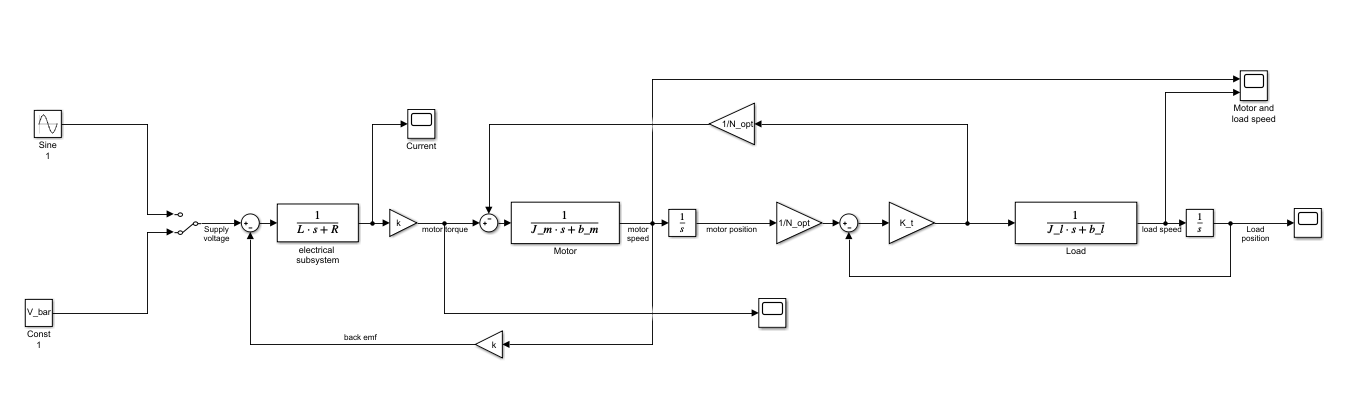
\includegraphics[width=150mm]{images/schema.png}
	\caption{Model of the beam}
	\label{scheme}
\end{figure}
In the Figure \ref{scheme} the Simulink model is shown. I imposed the external torque $\tau_l=0$ \\
Setting $K_t=10000~Nm/rad$ we get the following results:
\begin{figure}[H]
	\begin{subfigure}[b]{0.3\textwidth}
		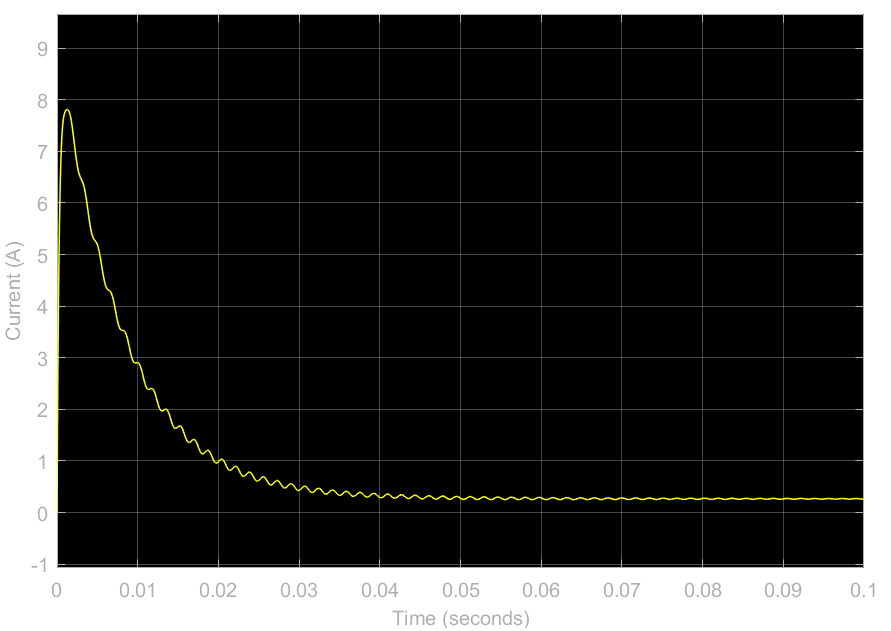
\includegraphics[width=50mm]{images/current1.png}
		\caption{Current}
	\end{subfigure}
	\hfill
	\begin{subfigure}[b]{0.3\textwidth}
		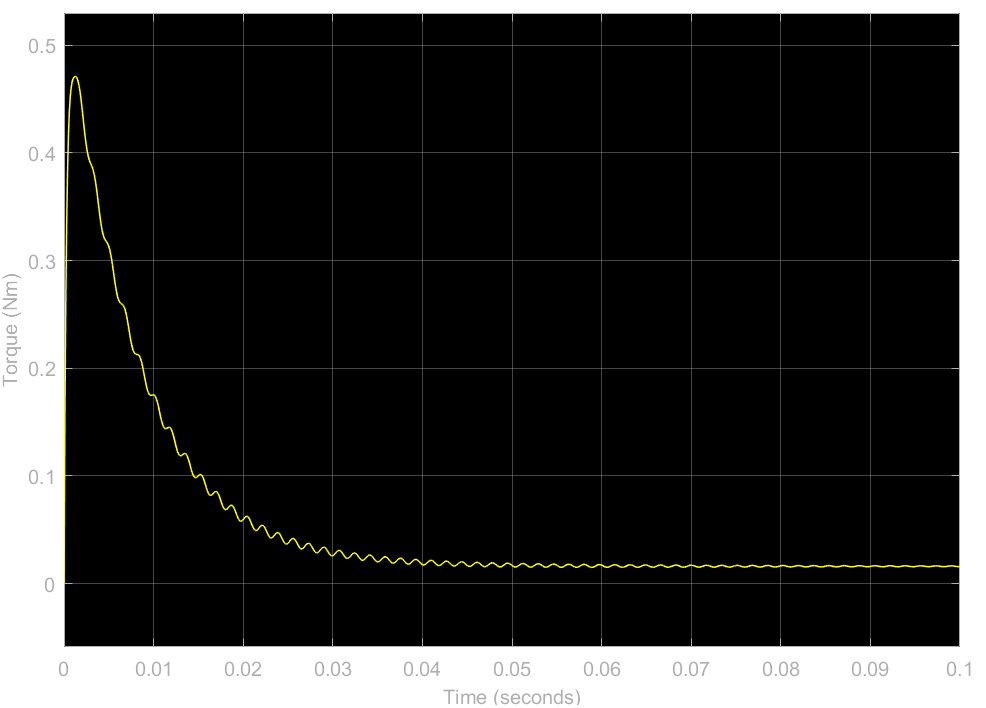
\includegraphics[width=50mm]{images/torque1.png}
		\caption{Motor torque}
	\end{subfigure}
	\hfill
	\begin{subfigure}[b]{0.3\textwidth}
		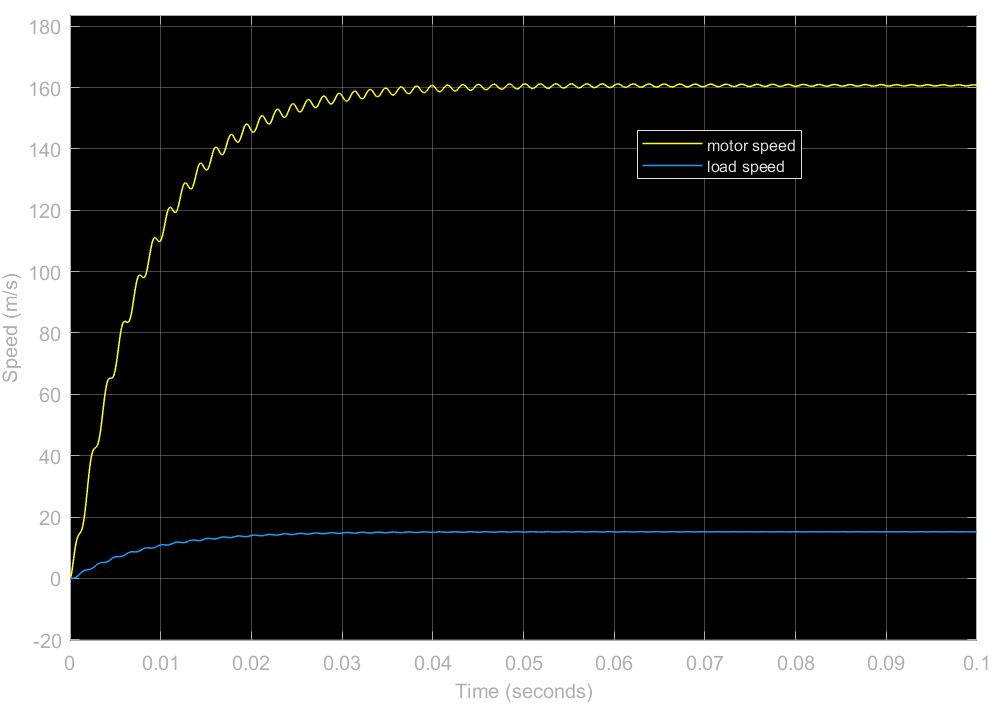
\includegraphics[width=50mm]{images/speed1.png}
		\caption{Motor and load speed}
	\end{subfigure}
	\caption{$K_t$ high: parameters behavior}
	\label{fig1}
\end{figure}
From the picture above little oscillations are visible in all 3 plots. To the eye they are bigger in motor speed respect to motor torque and current.

\newpage

Let's try to reduce the stiffness to $100~Nm/rad$:
\begin{figure}[H]
	\begin{subfigure}[b]{0.3\textwidth}
		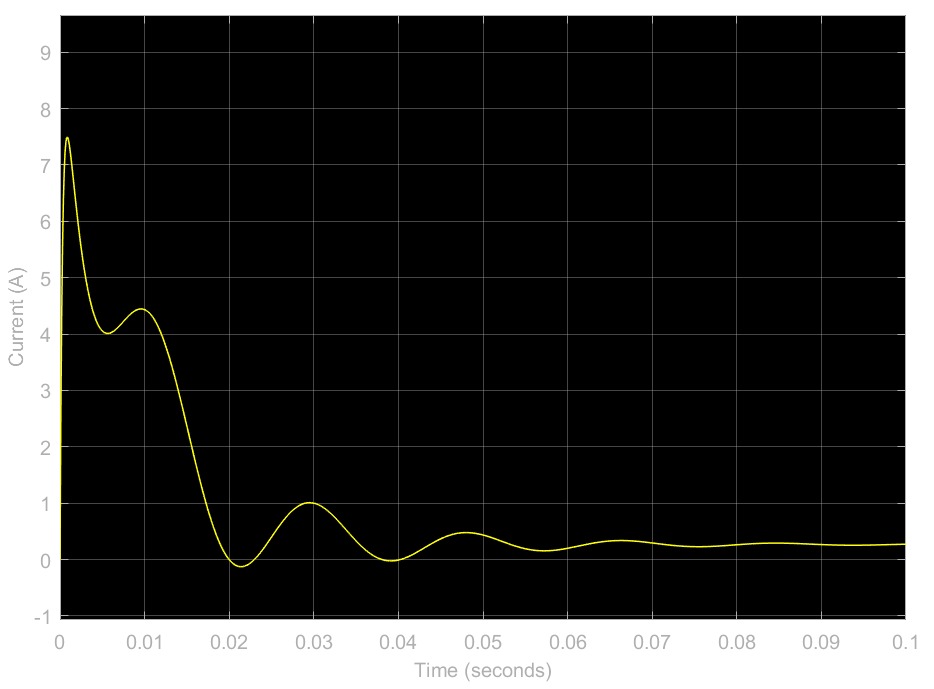
\includegraphics[width=50mm]{images/current2.png}
		\caption{Current}
	\end{subfigure}
	\hfill
	\begin{subfigure}[b]{0.3\textwidth}
		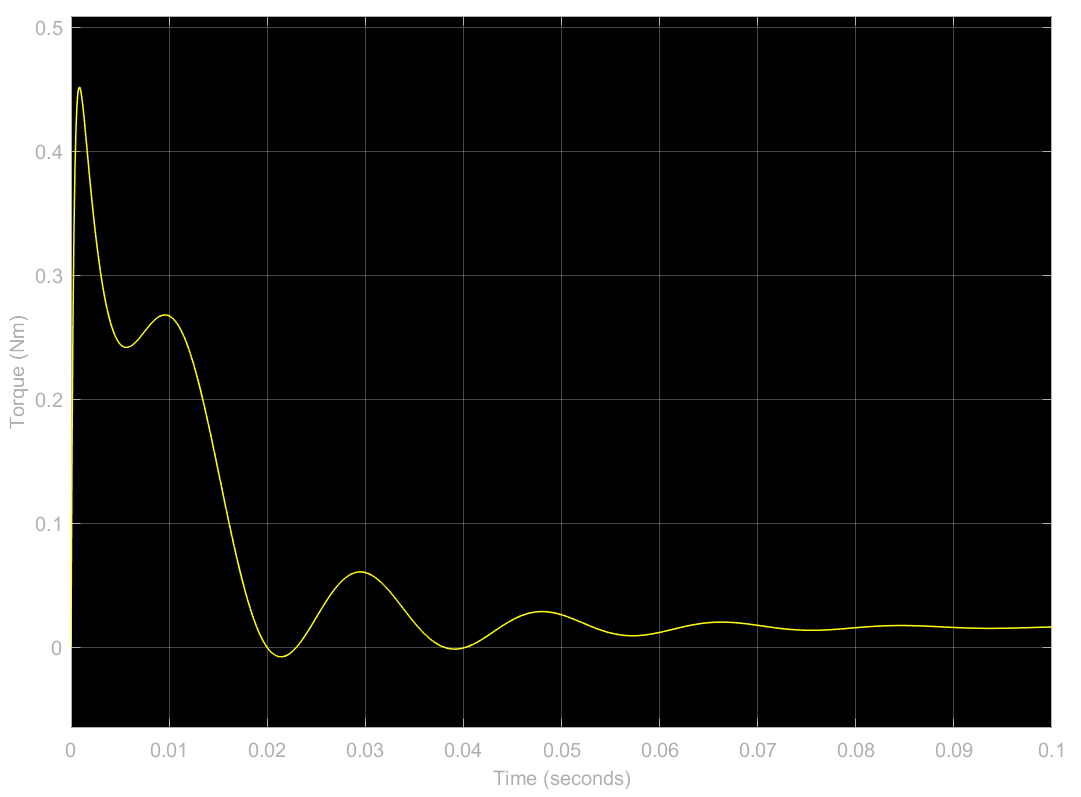
\includegraphics[width=50mm]{images/torque2.png}
		\caption{Motor torque}
	\end{subfigure}
	\hfill
	\begin{subfigure}[b]{0.3\textwidth}
		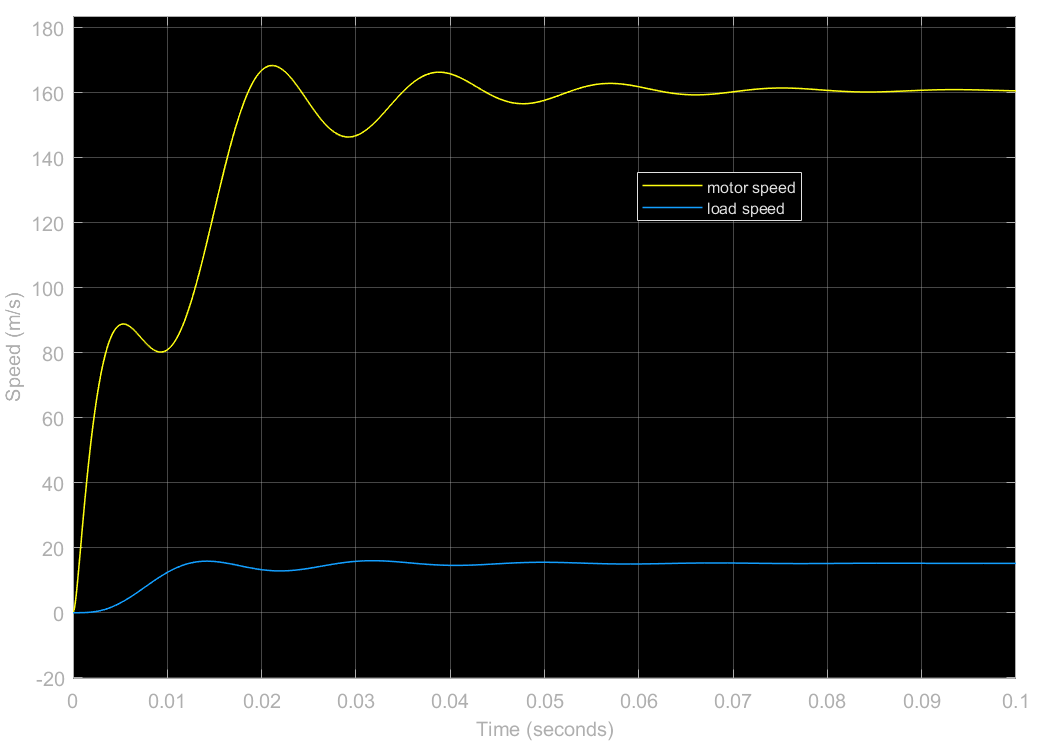
\includegraphics[width=50mm]{images/speed2.png}
		\caption{Motor and load speed}
	\end{subfigure}
	\caption{$K_t$ low: parameters behavior}
	\label{fig2}
\end{figure}
Reducing the stiffness of transmission oscillation increases significantly because the system becomes less stiff and more compliant. 
\section{PYTHON Exercise: Design a trajectory at the Cartesian level}	
Instead of computing the trajectory of the joints, we can do it at the end-effector level and then map to joint space by using inverse kinematics. \\
As initial and final point I selected respectively the one we obtained with direct kinematics of \texttt{conf.q0} and the desired point used later for inverse kinematics imposing $\Phi=0$ for both of them.

\smallskip

\texttt{start\_p = np.array([-0.68538, -0.11015, 0.5216, 0.0]) }\\
\texttt{end\_p   = np.array([-0.5, -0.2, 0.5, 0.0]) }

\smallskip

Velocity and acceleration has been initialized to 0.
\begin{figure}[H]
	\begin{subfigure}[b]{0.5\textwidth}
		\centering
		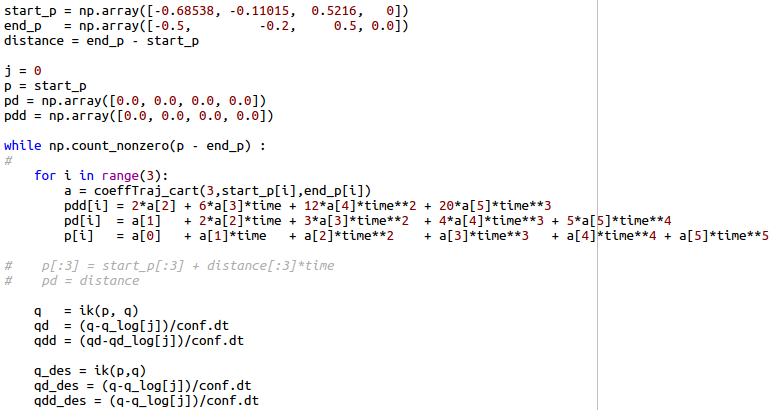
\includegraphics[width=65mm]{images/cod2_es2.png}
		\caption{Main code}
	\end{subfigure}
	\begin{subfigure}[b]{0.5\textwidth}
		\centering
		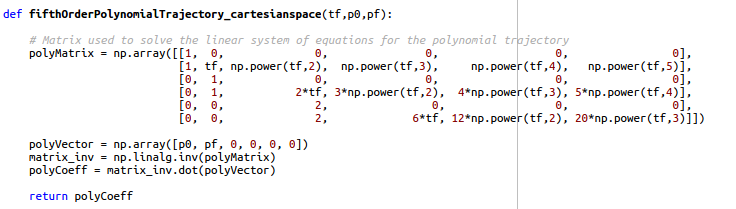
\includegraphics[width=65mm]{images/cod1_es2.png}
		\caption{Cartesian fifth order polynomial}
	\end{subfigure}
	\caption{Python code exercise 2}
	\label{codici}
\end{figure}
In order to design the trajectory, I tried two different approach: interpolating two points in the workspace keeping constant the velocity, and manage the function of the fifth order polynomial for the end-effector, but I am not sure of the results, honestly. 
Moreover velocity and acceleration was computed in a simplified manner with the difference of two consecutive values and dividing by the time step.
\begin{figure}[H]
	\begin{subfigure}[b]{0.33\textwidth}
		\centering
		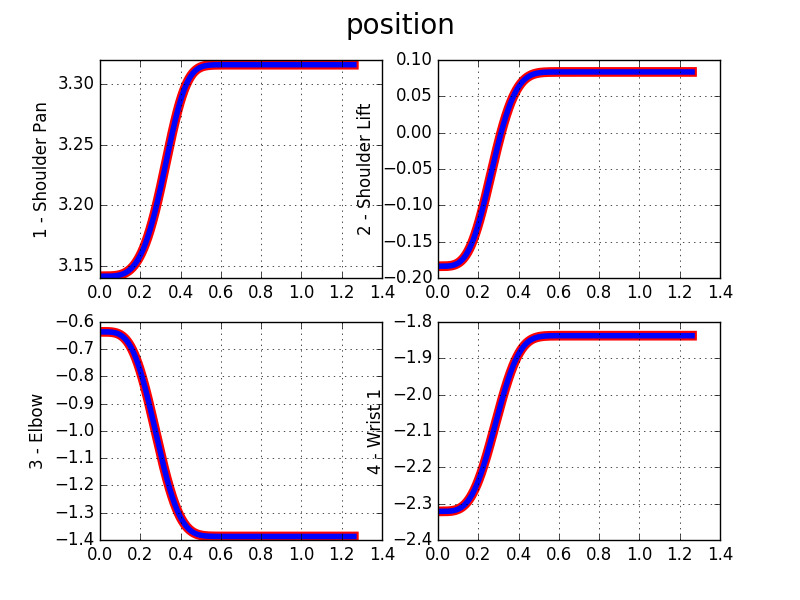
\includegraphics[width=50mm]{images/pos.JPEG}
		\caption{E-E Position}
	\end{subfigure}
	\begin{subfigure}[b]{0.33\textwidth}
		\centering
		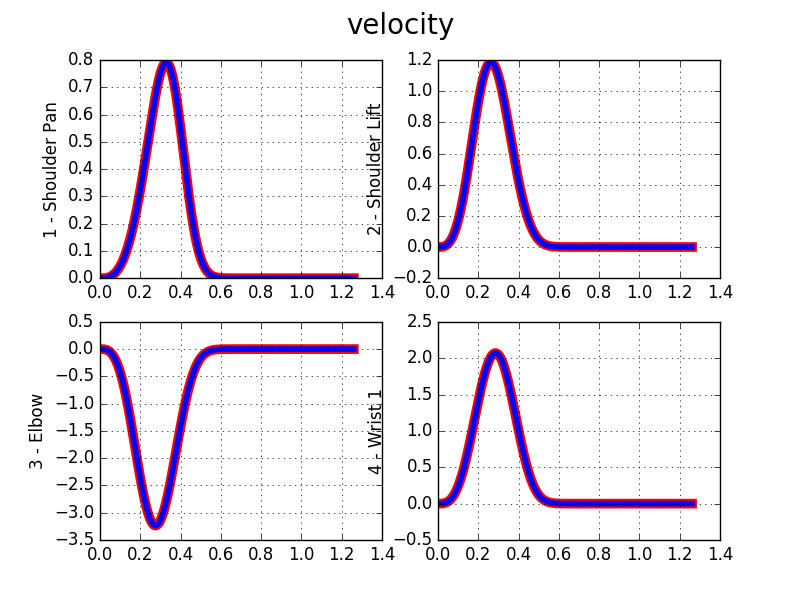
\includegraphics[width=50mm]{images/vel.JPEG}
		\caption{E-E Velocity}
	\end{subfigure}
	\begin{subfigure}[b]{0.33\textwidth}
		\centering
		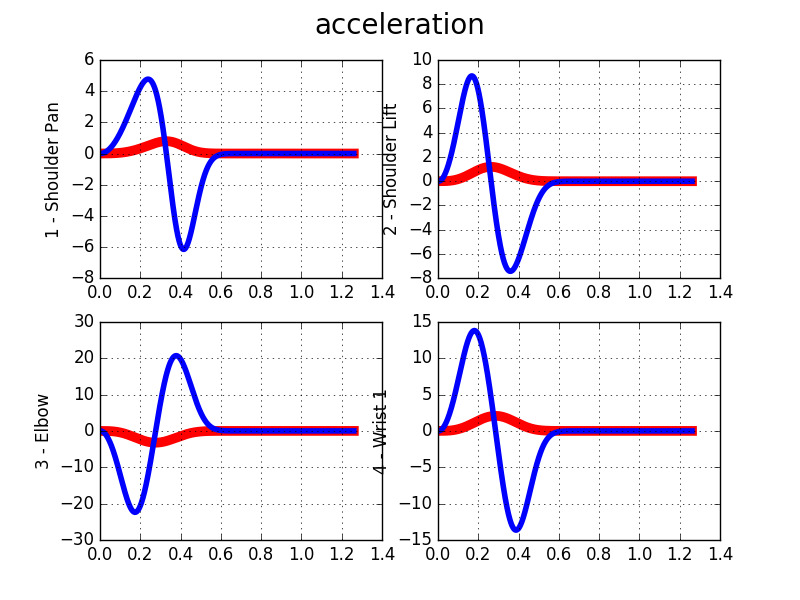
\includegraphics[width=50mm]{images/acc.JPEG}
		\caption{E-E Acceleration}
	\end{subfigure}
	\caption{Python code exercise 2}
	\label{codici}
\end{figure}
The plots show that position and velocity are tracked very well. You cannot say the same for the acceleration in which peaks which differ from the reference curve are present in the transient.  
\section{PYTHON Exercise: Inverse kinematics approach}	
I want to implement the end-effector tracking using inverse kinematics (with line search) to obtain the desired joint trajectory, and the pseudo-inverse Jacobian for velocity and acceleration. \\
In Figure \ref{codici} the code is shown: end-effector position and jacobian are computed with Pinocchio library; the Jacobian is a 3x6 fat matrix (x, y and z coordinates of the end-effector and 6 joints). For this reason the computation of Moore-Penrose pseudoinverse is $A^\dagger=A^T(AA^T)^{-1}$. Finally I used a PD control with feed-forward term and evaluate the tracking error.  
\begin{figure}[H]
	\begin{subfigure}[b]{0.5\textwidth}
		\centering
		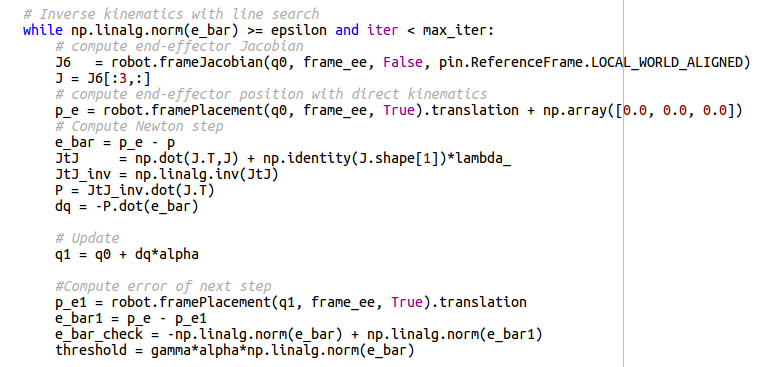
\includegraphics[width=65mm]{images/cod2_es3.png}
		\caption{Main code}
	\end{subfigure}
	\begin{subfigure}[b]{0.5\textwidth}
		\centering
		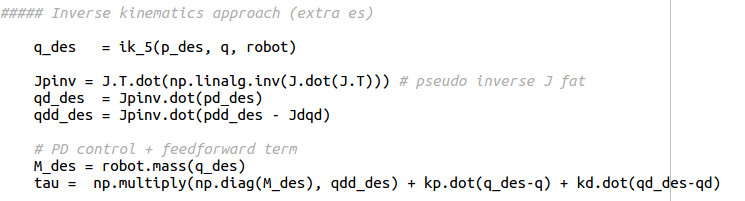
\includegraphics[width=65mm]{images/cod1_es3.png}
		\caption{Inverse kinematics function}
	\end{subfigure}
	\caption{Python code exercise 3}
	\label{codici}
\end{figure}

I assessed the performance of my controller with the predefined sinusoidal reference trajectory. In the next plots we can see the corresponding results.

\begin{figure}[H]
	\begin{subfigure}[b]{0.5\textwidth}
		\centering
		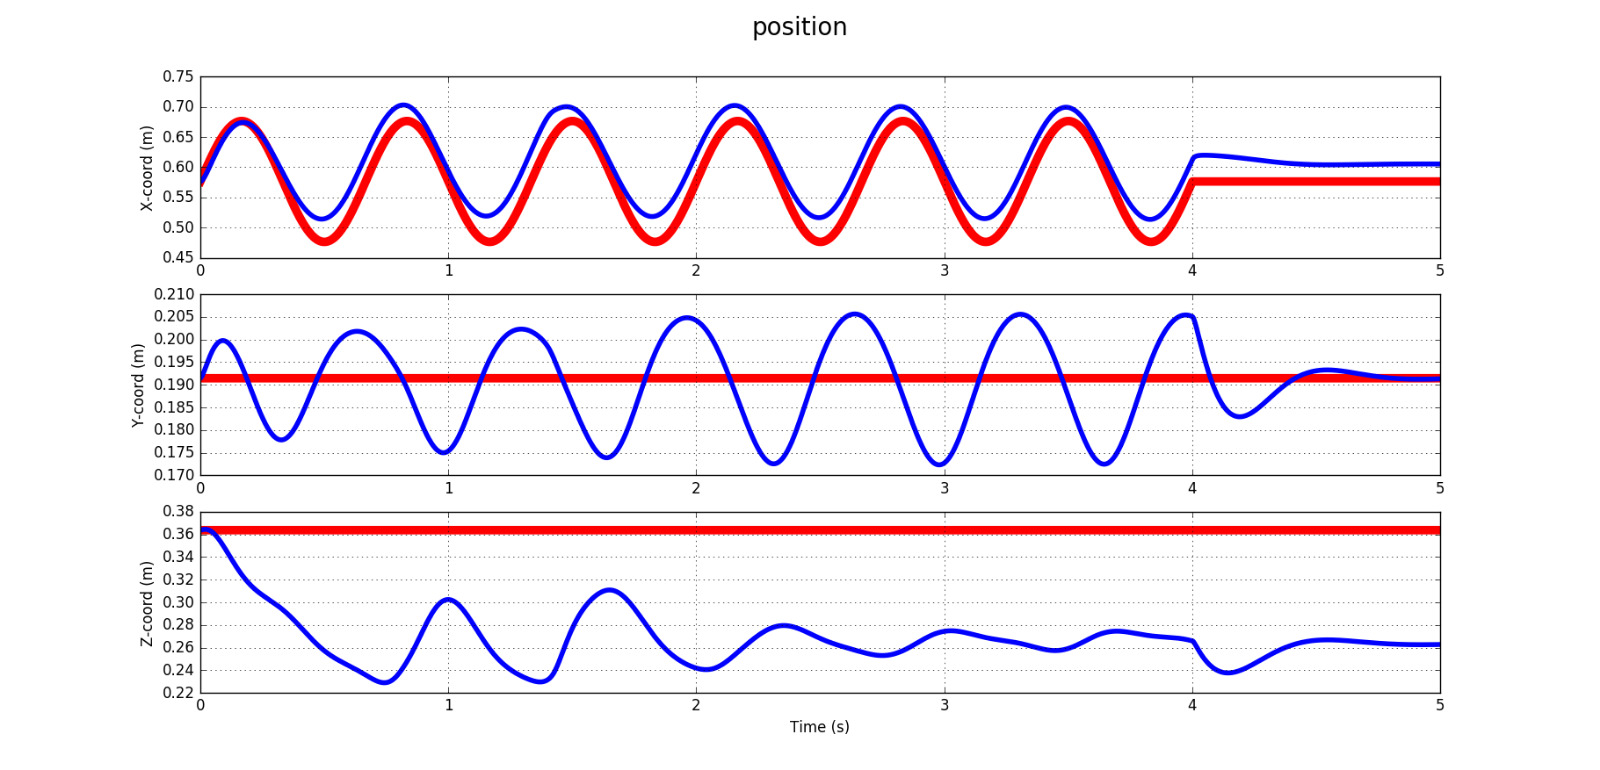
\includegraphics[width=75mm]{images/sineh.JPEG}
		\caption{PD control + FD term}
	\end{subfigure}
	\begin{subfigure}[b]{0.5\textwidth}
		\centering
		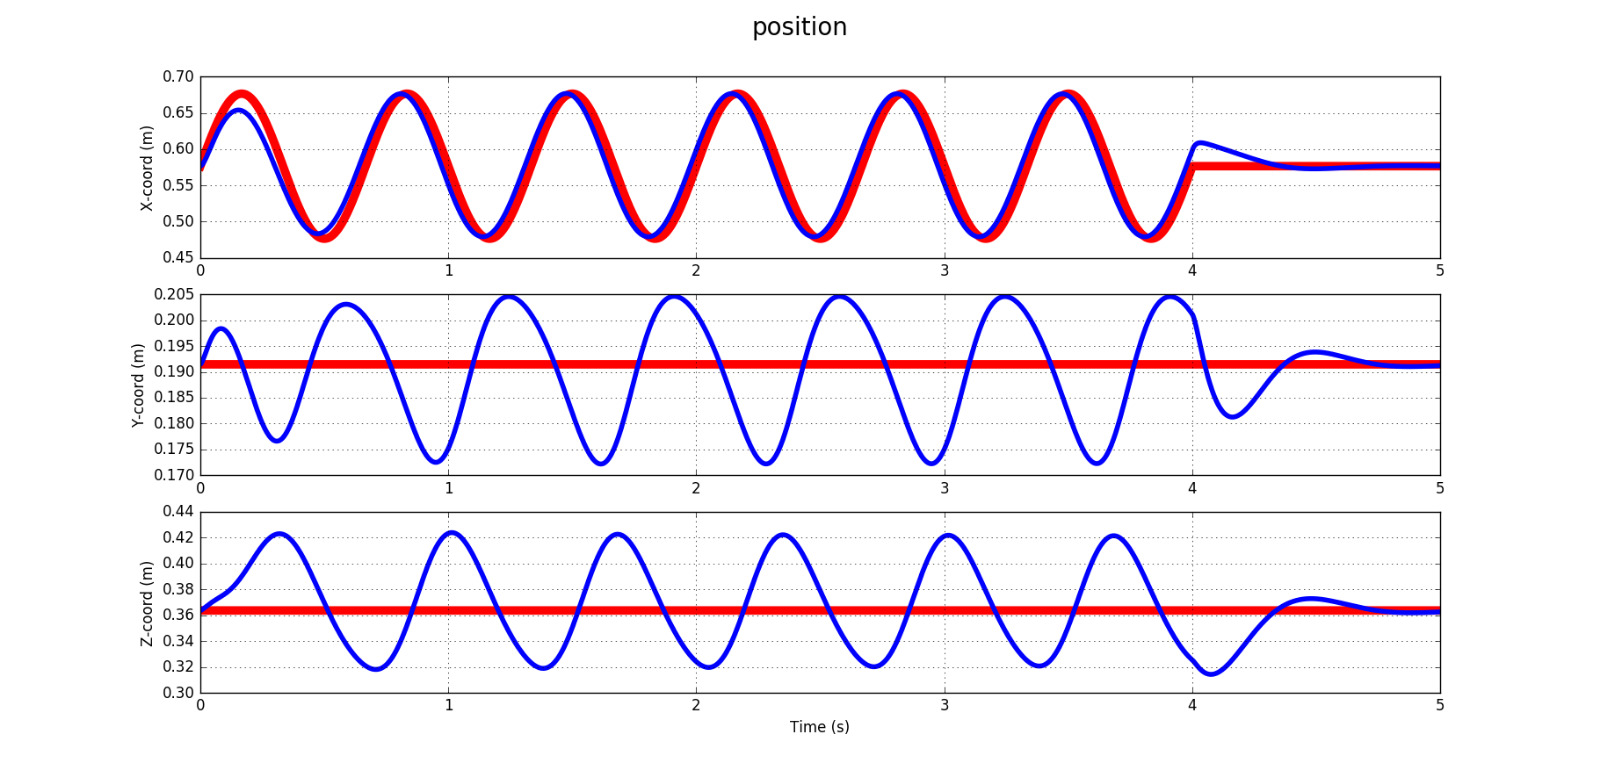
\includegraphics[width=75mm]{images/sine_g.JPEG}
		\caption{PD control + FD term + gravity compensation}
	\end{subfigure}
	\caption{End-effector position}
	\label{controller}
\end{figure}

\begin{figure}[H]
	\centering
	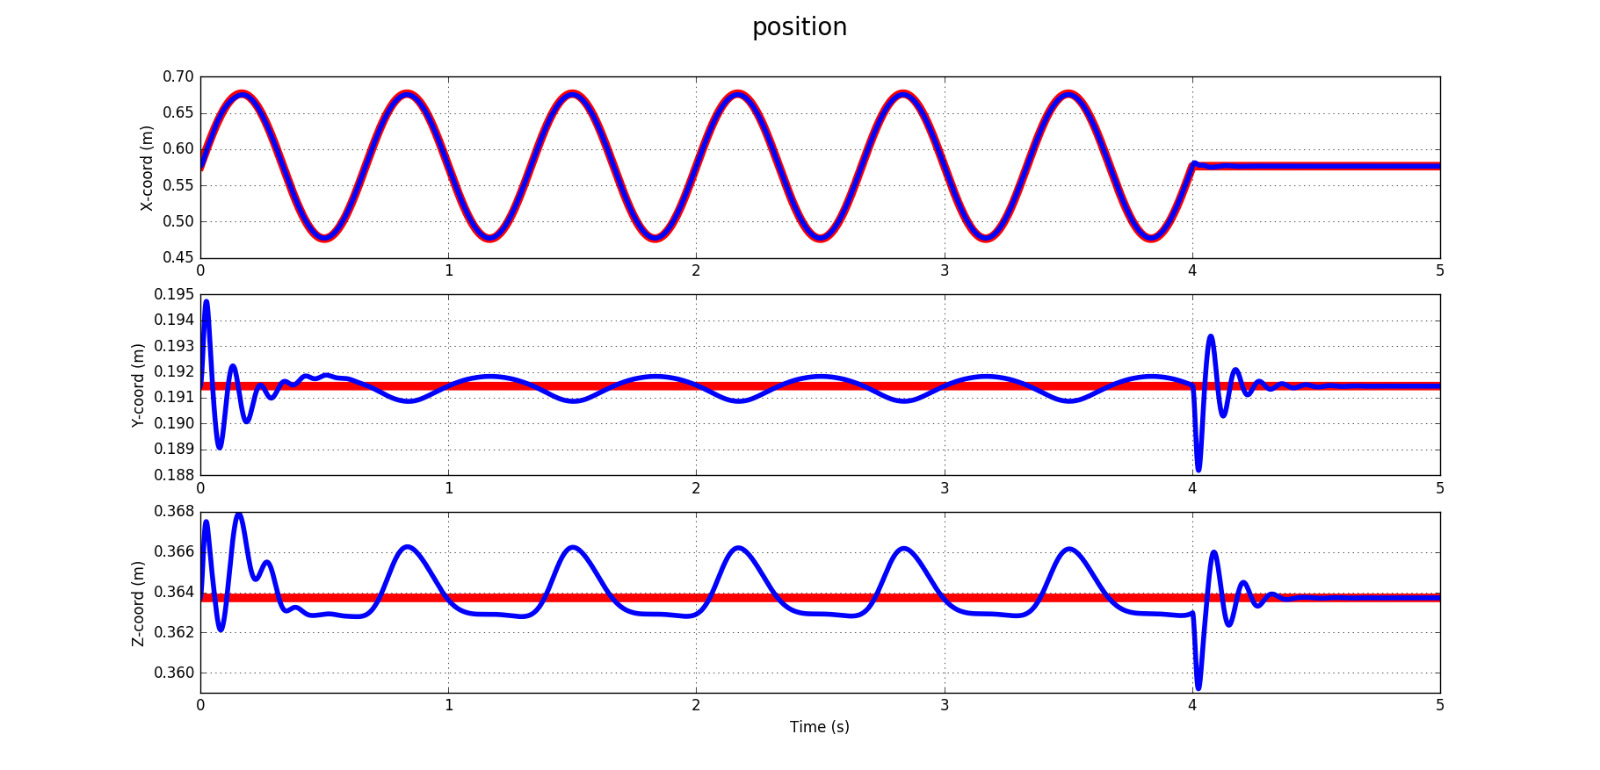
\includegraphics[width=100mm]{images/sine_kp.JPEG}
	\caption{$K_p=10000$}
	\label{plot3}
\end{figure}

Observing that for the z-coordinate the initial result was bad, I added a gravity compensation (Figure \ref{controller} (b)) which made the manipulator follow the trajectory. Not completely satisfied I increase the $K_p$ gain to 10000 and get the last plot.

 
\footnotesize
\newpage
\hypersetup{linkcolor = black}
\listoffigures
%\listoftables
\end{document}